\chapter{使用 STM32CubeMX 新建工程}
本章节将以最简单的 LED 亮灯需求为例, 展示如何用 STM32CubeMX 新建工程. 前文已有说明, 若仅为了学习本课程, 可以不使用此软件, 而是使用我们提供的空白工程编写程序. 当然, 我们的空白工程也是在 STM32CubeMX 生成的工程基础上改进而来的. 在本章节之后, 所有的 labs 涉及到的工程皆以我们提供的空白工程为基础.

启动 STM32CubeMX. 启动后可能会弹出如下图的下载窗口, 无视之, 可以放心直接点 Cancel.

\begin{figure}[H]
    \centering
    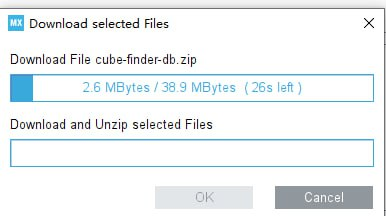
\includegraphics{images/1-newproj-down.jpg}
    \caption{STM32CubeMX 的下载窗口}
\end{figure}

\section{选择 CPU 型号}
根据开发板使用的 CPU 型号来选择. 以 F4 霸天虎为例, 应该选择 STM32F407ZGT6. 具体的流程是, 先依次点击左上角的 ``File''-``New Project ...'', 在弹出的窗口左上角搜索框输入型号, 再在右侧的条目中双击 ``STM32F407ZGT6''. 如下图所示.

\begin{figure}[H]
    \centering
    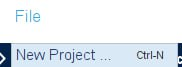
\includegraphics{images/1-newproj-new.jpg}
    \caption{STM32CubeMX 新建工程}
\end{figure}

\begin{figure}[H]
    \centering
    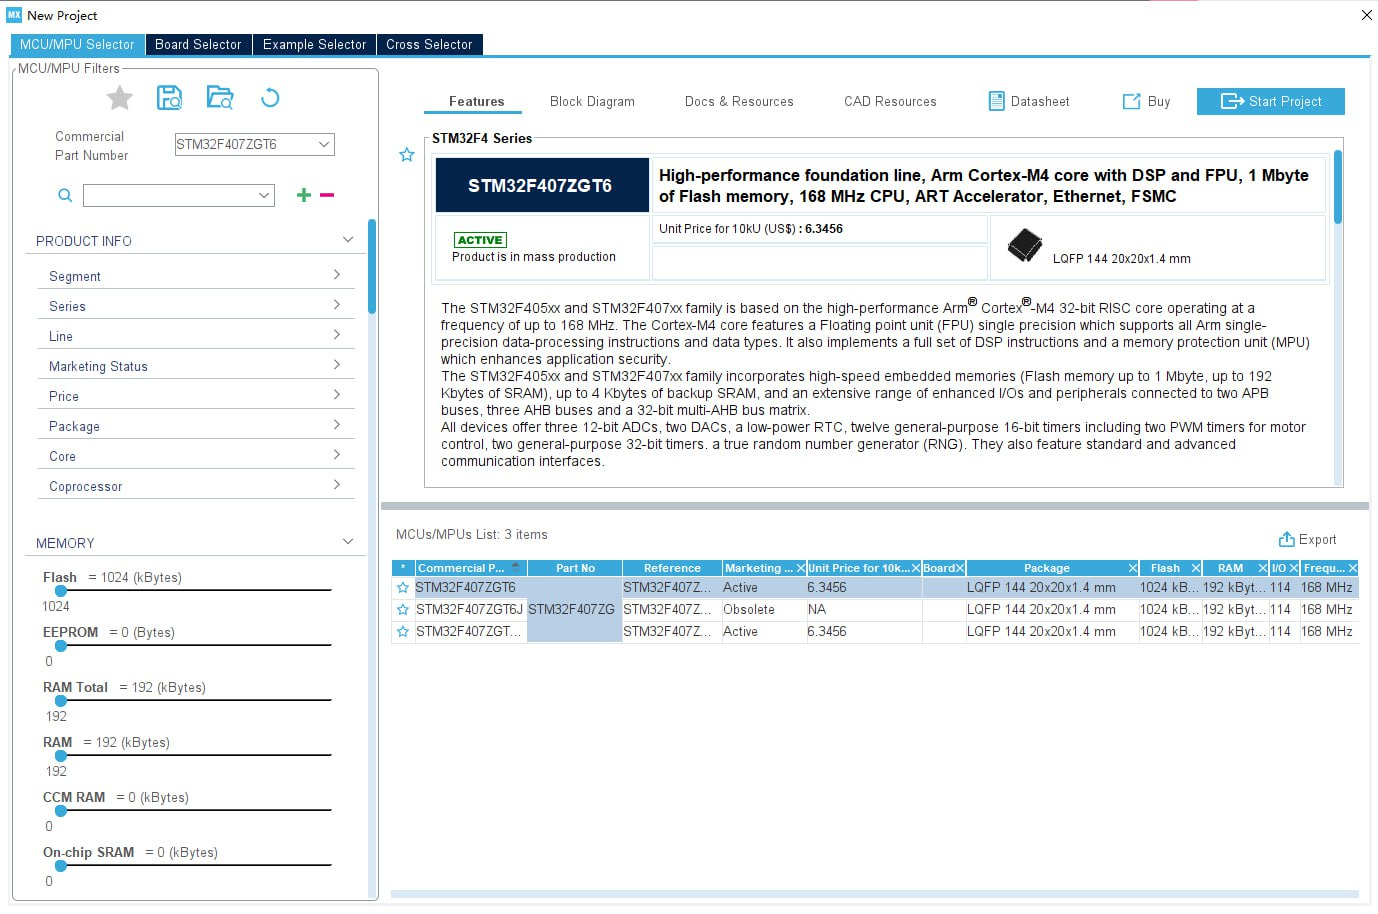
\includegraphics[width=\textwidth]{images/1-newproj-selectmodel.jpg}
    \caption{STM32CubeMX 选择 CPU 型号}
\end{figure}

\section{配置 IO 口}
这是属于硬件设计的一部分, 但是在软件设计中也需有所知晓. 虽然这一步可以跳过, 但是这样可以节省一些编写代码的时间成本.

我们需要根据我们的实际需求, 选择所需要的 IO 口. 对于本章节的示例, 通过查阅如下的本开发板的原理图, 可以知道 LED 红灯的外设所连接的 GPIO 口为 PF6, 因此只需在软件中配置该口即可.

\begin{figure}[H]
    \centering
    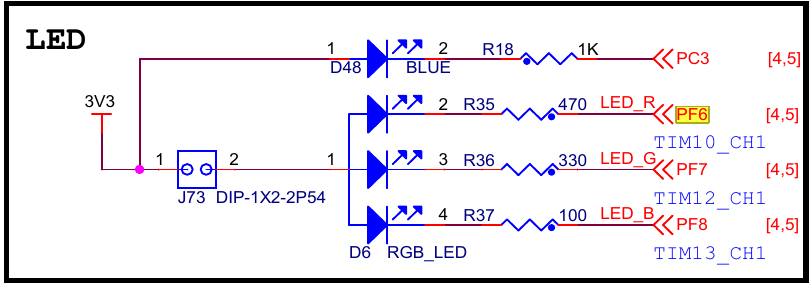
\includegraphics[width=.8\textwidth]{images/1-newproj-led.png}
    \caption{STM32F407ZGT6 的 LED 模块原理图}
\end{figure}

在软件显示的窗口中, 在右侧的芯片示意图上找到 PF6 引脚, 或者在下方的搜索框中搜索该引脚. 找到该引脚后, 左键单击将弹出一个小菜单, 这表明我们可以对其配置的用途类型. 因为我们需要用 GPIO 控制它的电平, 所以点击 ``GPIO\_Output''. 之后这个引脚会显示绿色背景色, 表示设置成功. 具体如下图所示.

\begin{figure}[H]
    \centering
    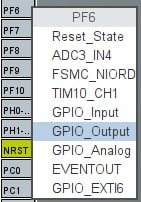
\includegraphics{images/1-newproj-setpin.jpg}
    \caption{STM32CubeMX 配置引脚}
\end{figure}

之后我们需要配置它的一些其他信息 (当然保持默认而略过这个步骤同样是可以的). 点击上方的 ``System view'', 点击中间的 ``GPIO'', 在弹出的左侧窗口中找到 ``PF6'' 条目, 在下方的 ``PF6 Configuration :'' 中可以配置 GPIO 的输出信号 (高电平还是低电平), GPIO 模式 (Push-Pull 推挽输出还是 Open-Drain 开漏输出) 等, 我们这里保持默认即可. 另外可以在下方设置 ``User Label'', 这样方便我们使用这个 label 的名字调用 GPIO (实质上是用宏定义了这个引脚的 port 和 pin). 如下图所示.

\begin{figure}[H]
    \centering
    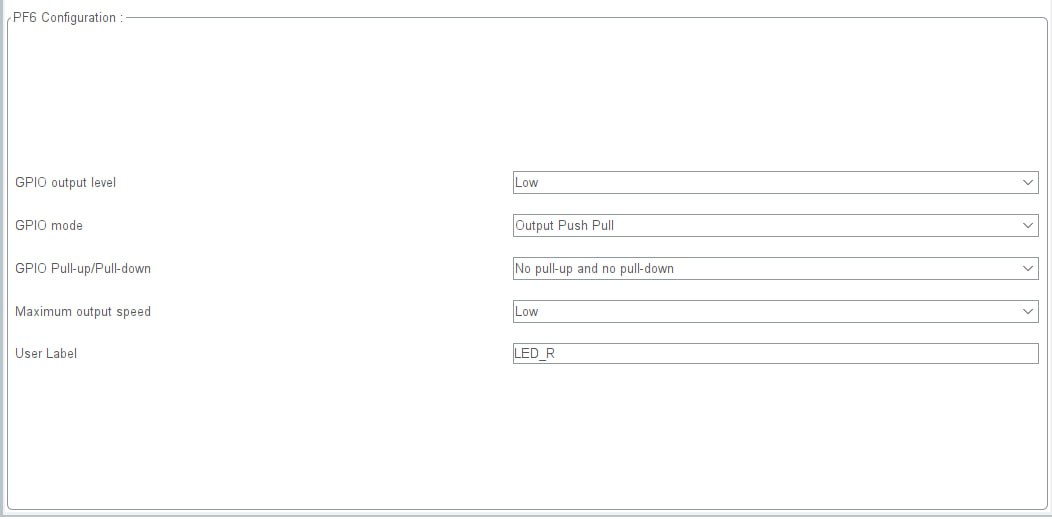
\includegraphics[width=\textwidth]{images/1-newproj-configpin.jpg}
    \caption{STM32CubeMX 配置引脚详细信息}
\end{figure}

\section{配置工程属性及下载硬件包}
点击上方的 ``Project Manager'', 我们首先设置的是上方的 ``Project Name'' (注意路径都不能包含中文或空格) 和 ``Toolchain Folder Location'', 其中前者表示这个工程的名字, 后者表示工程存放的位置. 随后下方的 ``Toolchain / IDE'' 下拉框选择 ``Makefile''. 如下图所示.

\begin{figure}[H]
    \centering
    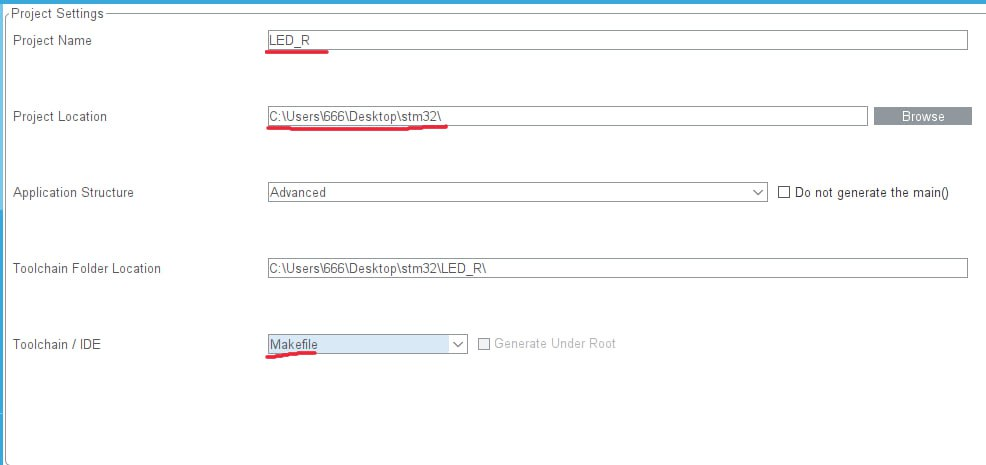
\includegraphics[width=\textwidth]{images/1-newproj-configproj.jpg}
    \caption{STM32CubeMX 配置工程信息}
\end{figure}

中间的设置保持默认. 最后我们设置最下方的 ``Mcu and Firmware Package''. 我们将不使用 STM32-CubeMX 自带的下载工具来下载硬件包, 而是选择从 GitHub 获取. 先观察下方 ``Firmware Relative Path'' 的路径格式, 其应该类似于 \texttt{/path/to/STM32Cube/Repository/xxx}, 如下图所示.

\begin{figure}[H]
    \centering
    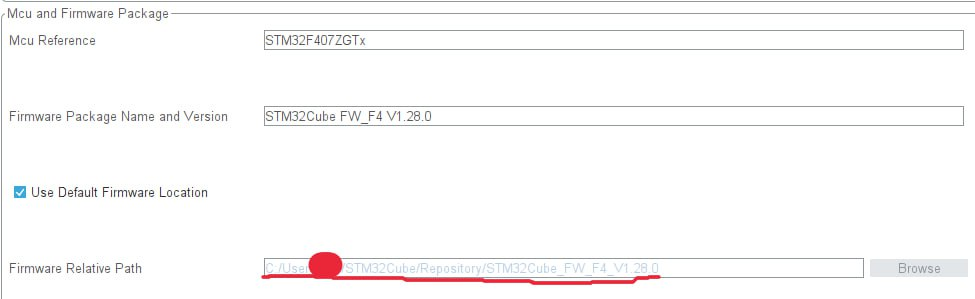
\includegraphics[width=\textwidth]{images/1-newproj-configfirm.jpg}
    \caption{STM32CubeMX 的 Mcu and Firmware Package 设置}
\end{figure}

接着, 我们在终端中执行如下的命令:

\begin{minted}{bash}
mkdir -p /path/to/STM32Cube/Repository
cd /path/to/STM32Cube/Repository
git clone --recursive https://github.com/STMicroelectronics/STM32CubeF4.git xxx # 记得替换 xxx 为真实的路径!
\end{minted}

这样我们就配置好了硬件包, 之后每次新建工程都不需要修改硬件包的路径了.

\section{测试工程}
所有都配置好后, 我们点击右上角的 ``GENERATE CODE'' 生成代码. 等待代码生成完成后, 在终端进入工程所在文件夹, 在终端中执行 \texttt{make} 编译. 编译完成后, 我们应当能在 \texttt{build/<工程名>.bin} 找到编译出的文件. 接着, 用专用线将电脑 USB 和开发板串口连接, 在开发板进入 bootloader 模式后, 在终端中执行

\begin{minted}{bash}
sudo stm32flash -w build/<工程名>.bin -v -g 0x0 /dev/ttyUSB0
\end{minted}

待程序烧录完成后, 引导开发板进入主闪存存储器启动模式, 此时可以看到 LED 常亮红灯, 表示开发环境和工程测试成功.
